\documentclass{article}
\usepackage[T1]{fontenc}
\usepackage[dvipsnames]{xcolor}
\usepackage{tikz}
\usetikzlibrary{positioning,arrows.meta}
\usepackage{amsmath}
\usepackage{amssymb}
\usepackage{xcolor}

\begin{document}

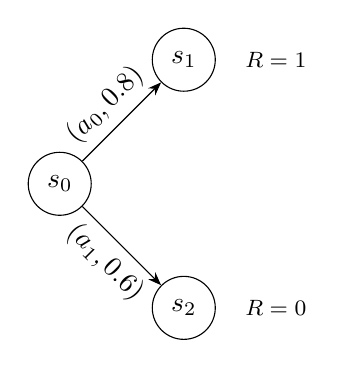
\begin{tikzpicture}[auto,
vertex/.style={minimum size=0.8cm,draw,circle,text width=0.8mm},
]%
    \node[vertex,label=center:$s_{0}$] (s0) {};
    \node[vertex,above right=1cm and 1cm of s0,label=center:$s_1$] (s1) {}; %
    \node[right=0.25cm of s1] (r1) {\footnotesize $R=1$};
    \node[vertex, below right= 1cm and 1cm of s0, label=center:$s_2$] (s2) {};
    \node[right=0.25cm of s2] (r2) {\footnotesize $R=0$};

     \path[-{Stealth[]}] %
      (s0) edge node[sloped, anchor=center,align=center,above] {$(a_0, 0.8)$} (s1)
      (s0) edge node[sloped, anchor=center,align=center,below] {$(a_1, 0.6)$} (s2)
    ;

\end{tikzpicture}

\end{document}